%%%%%%%%%%%%%%%%%%%%%%%%%%%%%%%%%%%%%%%%%
% Short Sectioned Assignment
% LaTeX Template
% Version 1.0 (5/5/12)
%`
% This template has been downloaded from:
% http://www.LaTeXTemplates.com
%
% Original author:
% Frits Wenneker (http://www.howtotex.com)
%
% License:
% CC BY-NC-SA 3.0 (http://creativecommons.org/licenses/by-nc-sa/3.0/)
%
%%%%%%%%%%%%%%%%%%%%%%%%%%%%%%%%%%%%%%%%%

%----------------------------------------------------------------------------------------
%	PACKAGES AND OTHER DOCUMENT CONFIGURATIONS
%----------------------------------------------------------------------------------------

\documentclass{article}

\usepackage[T1]{fontenc} % Use 8-bit encoding that has 256 glyphs
%\usepackage{fourier} % Use the Adobe Utopia font for the document - comment this line to return to the LaTeX default
\usepackage[english]{babel} % English language/hyphenation
\usepackage{amsmath,amsfonts,amsthm, amssymb} % Math packages
\usepackage{sectsty} % Allows customizing section commands
\usepackage{tikz-cd} % Allows for commutative diagrams
\usepackage[]{enumerate} %Changing enumerate environment
\usepackage{mathrsfs} %fonts?
\usepackage{cancel} % for pretty slashes
\usepackage{graphicx}

\begin{document}
	
	\title{Combinatorics and Computation Notes}
	\author{Nate Schieber}
	\date{11/11/2019}
	\maketitle
	
	\section{Example: Aztec Diamond Graph}
	
\hspace{1cm} We begin with an example of the Kasteleyn matrix using a bipartite Aztec Diamond graph of order 2, as shown in Figure \ref{fig:ad2}. Let $G = (V,E)$ be this graph and let the sign function $\sigma: E \rightarrow \{\pm 1\}$ be defined by the figure with unlabelled edges mapping to $+1$. Note that this map satisfies the defining property that
$$
\prod_{i=1}^{2k} \sigma(e_i) = 
	\begin{cases}
		1 & k \hspace{1mm} \text{odd} \\
		-1 & k \hspace{1mm} \text{even} 
	\end{cases}
$$
for each face $F = \{e_1, \dots, e_{2k}\}$ defined by $G$. 
\begin{figure}[h]
	\begin{center}
 	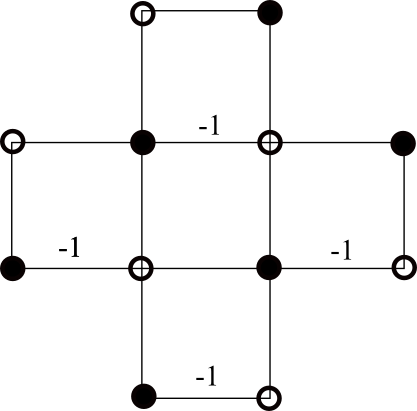
\includegraphics[width=6cm]{figures/aztec_diamond_2.png}
  	\caption{A Bipartite Aztec Diamond of Order 2}
	 \label{fig:ad2}
 	 \end{center}
\end{figure}

We can also consider the order $n$ Aztec Diamond graph. Figure \ref{fig:ad3} shows the case $n = 3$. 
\begin{figure}[h]
	\begin{center}
 	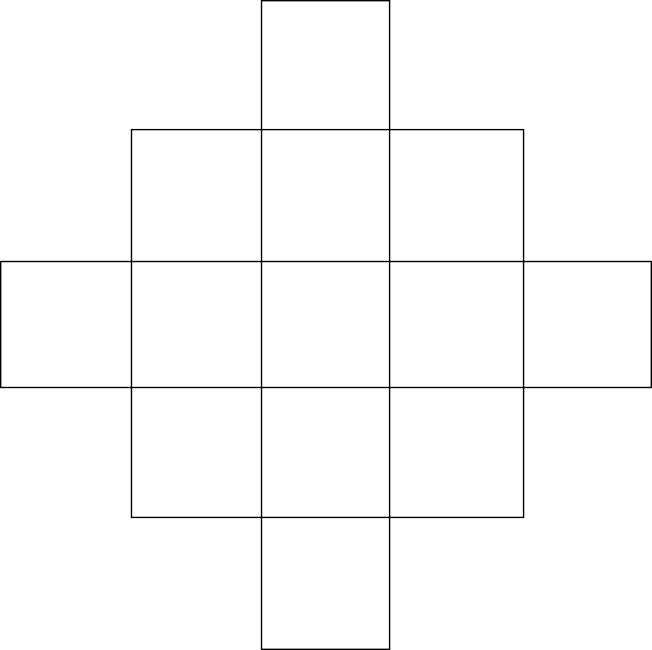
\includegraphics[width=4cm]{figures/aztec_diamond_3.png}
  	\caption{Aztec Diamond of Order 3}
	 \label{fig:ad3}
 	 \end{center}
\end{figure}
In general, the order $n$ Aztec Diamond graph has 
$$
2^{{n+1}\choose{2}} \hspace{1cm} \text{perfect matchings.}
$$


\section{Edge - Placement Probability}

\hspace{1cm} We now study the probability that a given edge in a bipartite graph appears in a random perfect matching. Specifically, let $G = (V = V_\bullet \amalg V_\circ, E)$ be an embedded, planar, bipartite graph. We assume that $G$ has perfect matchings, so in particular $\vert V_\bullet \vert = \vert V_\circ \vert$. 

Let $K$ be its Kasteleyn matrix so that $K$ is an $\vert V_\bullet \vert \times \vert V_\circ \vert$ matrix whose rows are indexed by black vertices and columns by white vertices. Then 
$$
\vert \det K \vert = \#\{ \text{perfect matchings on \hspace{.1cm}} G\}. 
$$

Suppose $e \in E$. We would like to know how to compute $\mathbb{P} \{e \in M\}$ where $M$ is a uniformly random perfect matching on $G$. 

\subsection{Motivation}

\hspace{1cm} Let us see how this probability arises in studying Aztec Diamonds. Inspection shows that for large $n$, uniformly random perfect matchings on the Aztec Diamond tend to follow a particular patter as shown in Figure \ref{fig:adl}. Within the circle, the matching $M$ appears random. However, outside of the circle, we find a remarkably regular ``frozen grid'' pattern. 
\begin{figure}[h]
	\begin{center}
 	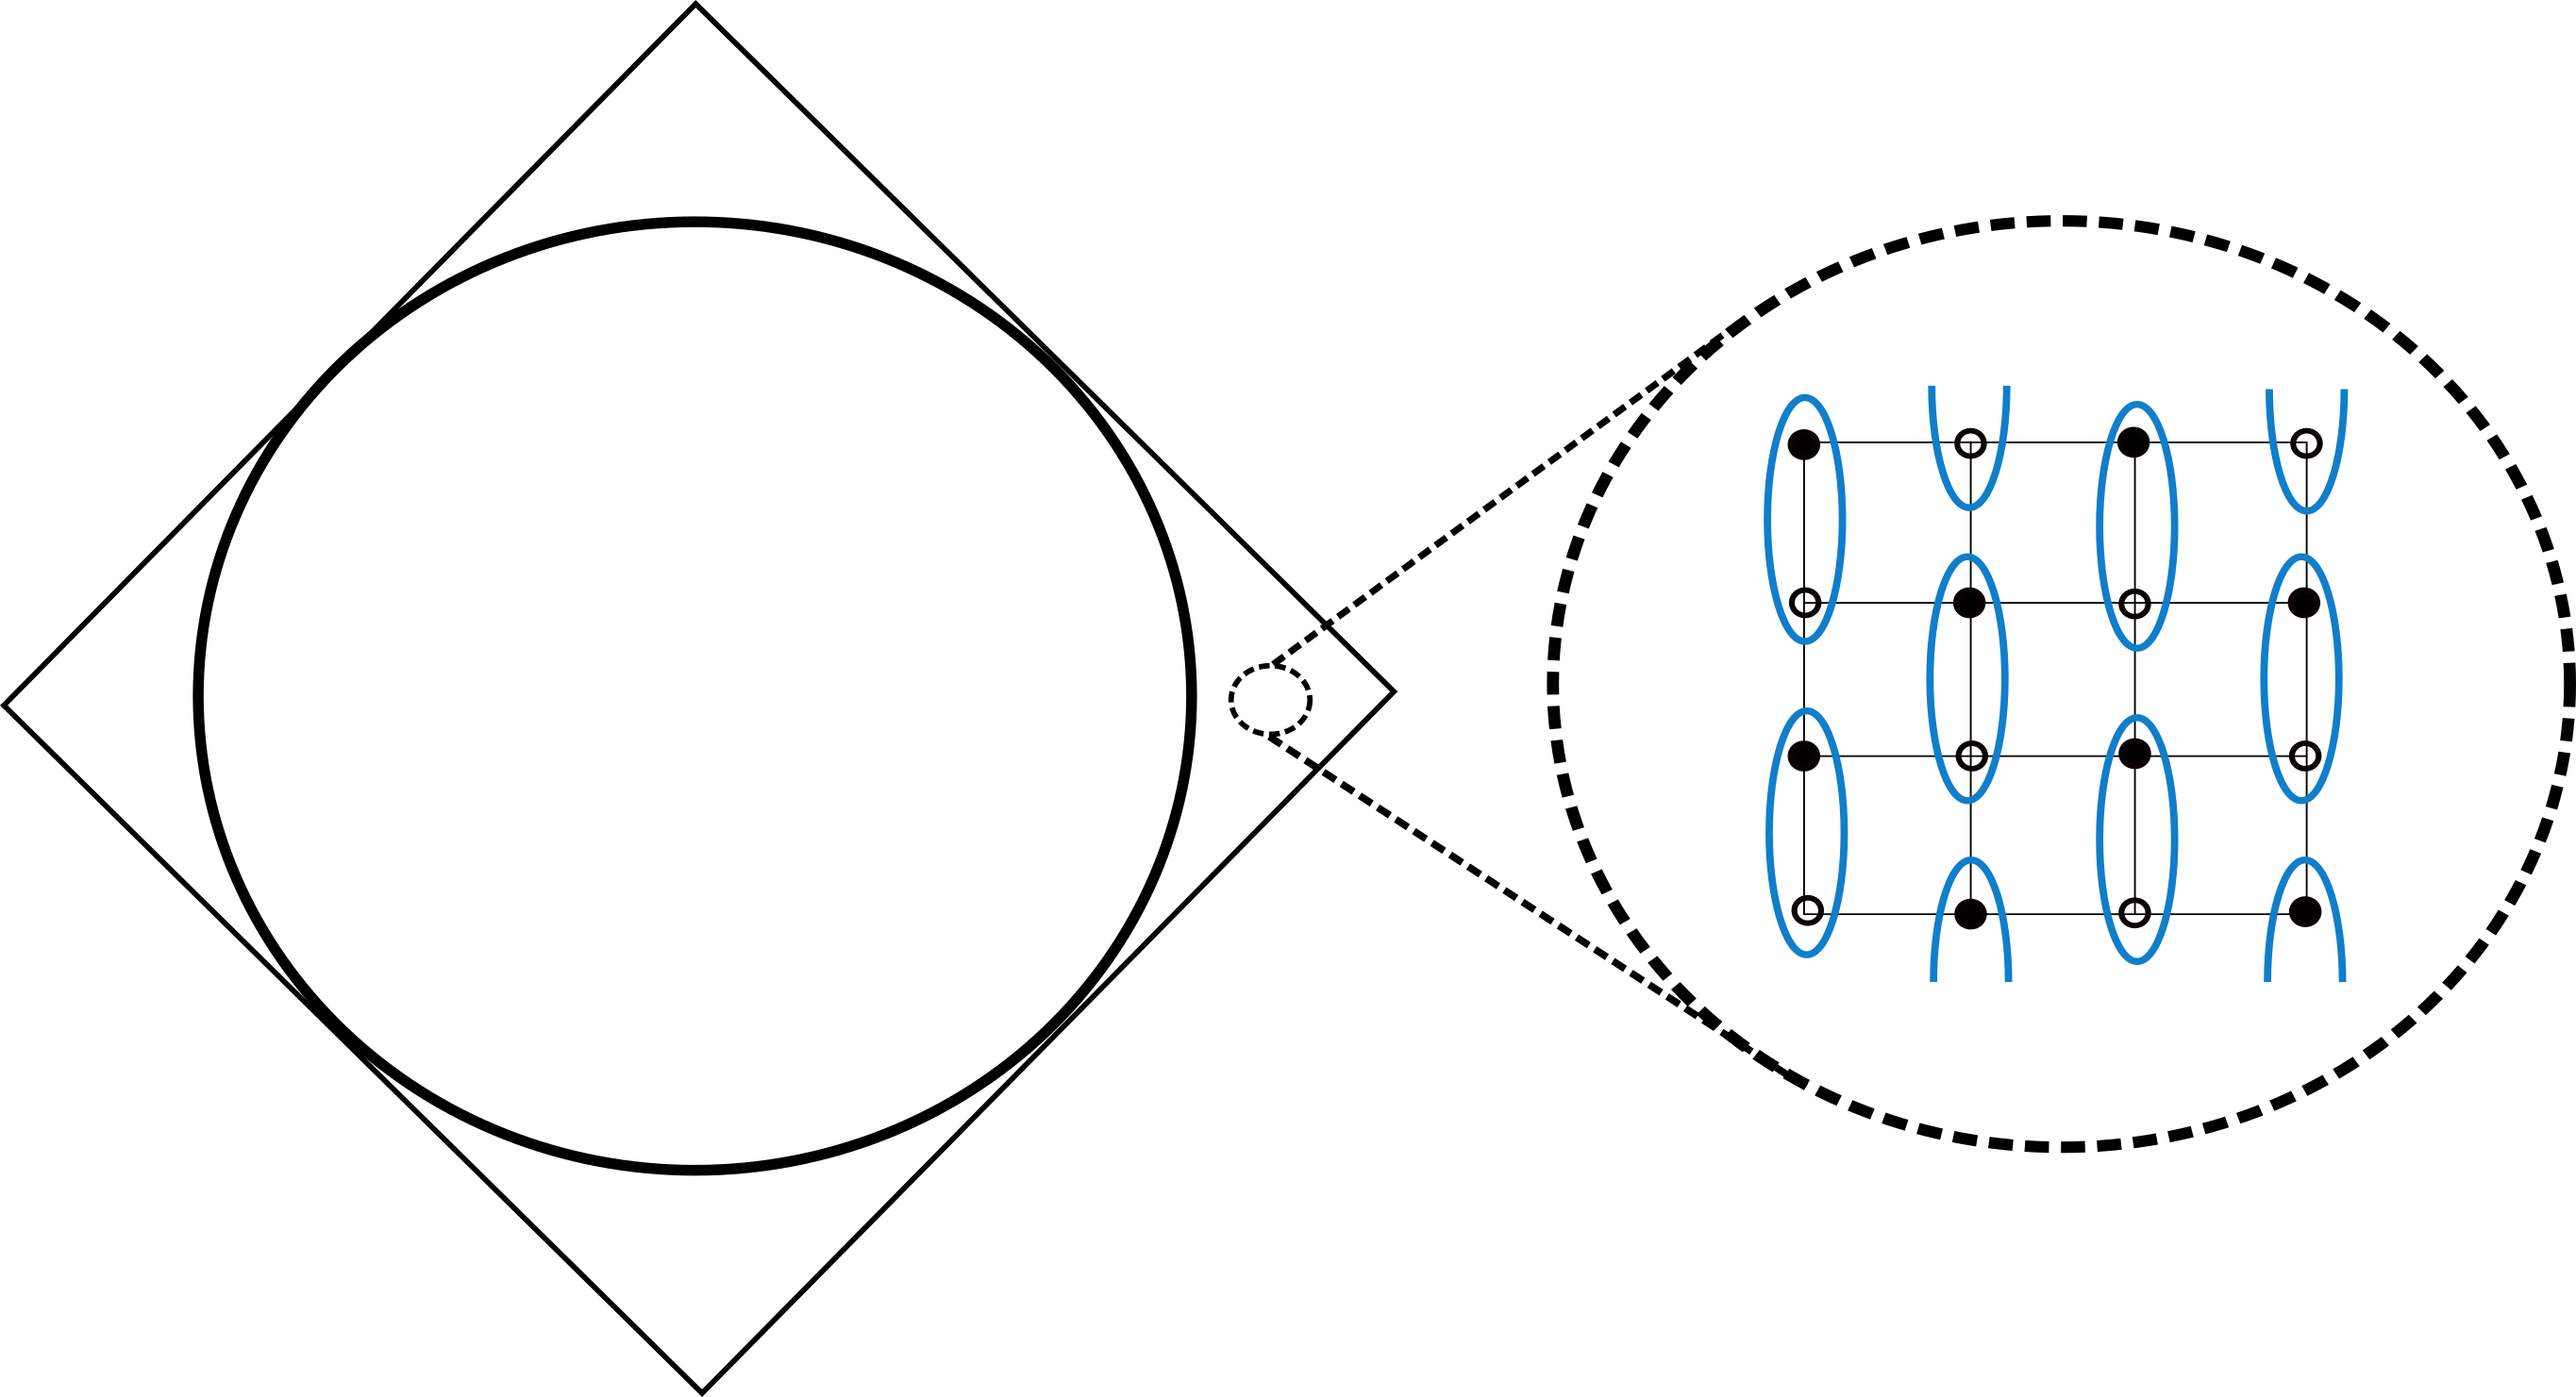
\includegraphics[width=7cm]{figures/aztec_diamond_limit.png}
  	\caption{Aztec Diamond Limit Patter}
	\label{fig:adl}
 	 \end{center}
\end{figure}

It can be shown that as $n \rightarrow \infty$ the probability of this pattern occurring goes to $1$. To show this, we compute
$
\mathbb{P} \{ e \in M\}
$
for a fixed horizontal edge $e$ near the boundary of the Aztec Diamond. We eventually find that $\mathbb{P} \{ e \in M\} \rightarrow 0$ as $n \rightarrow \infty$, thus leaving only vertical edges. 

\subsection{Computation}

\hspace{1cm} Let us compute the desired probability. Set $G,E,V,$ and $M$ as before. Let $e \in E$ be arbitrary. We have
$$
\mathbb{P} \{ e \in M\} = \frac{\# \{M \mid e \in M\}}{\# \{ M\}} = \frac{\# \{M \mid e \in M\}}{\vert \det K \vert}.  
$$
We must determine $\# \{ M \mid e \in M\}$. 

Define $G' = (V', E')$ where
$$
V' = V \smallsetminus \{\text{endpoints of}\hspace{.1cm} e \}
\hspace{.5cm} \text{and} \hspace{.5cm}
 E' = E \smallsetminus \left(\{e\} \cup \{\text{all edges incident to}\hspace{.1cm} e \} \right).
 $$
 Let $M'$ represent a perfect matching on $G'$. Then 
 $$
 \# \{M \mid e \in M\} = \#\{M'\}. 
 $$
The equality is easily observed by drawing a minimal example. 

We note that, as $G$ is bipartite, the vertices removed from $V$ are of opposite colors. Removing them thus corresponds to removing one column and one row from $K$. It can be shown that the resulting matrix $K'$ is indeed the Kasteleyn matrix for $G'$. 

With this in mind, suppose that $e$ has endpoints $(a,b) \in V_\bullet \times V_\circ$. Then $K' = K^b_a$, denoting $K$ with row $a$ and column $b$ removed.  We thus have
$$
 \#\{M'\} = \vert \det K^b_a \vert 
$$
whence
$$
\mathbb{P}\{e \in M\} = \frac{\vert \det(K^b_a) \vert}{\vert \det(K)\vert} = \vert (K^{-1})_{ba}\vert
$$
where $(K^{-1})_{ba}$ denotes the $ba$th entry of $K$ inverse. The right-most equality follows from Cramer's Rule. In words, the probability that a given edge $e$ in a bipartite, planar graph $G$, with endpoints $a \in V_\bullet$ and $b \in V_\circ$ is equal to the $ba$th entry of $K^{-1}$. 


\newpage

\section{Dimers and Spanning Trees (Temperley Map)}

\hspace{1cm} We will now observe a connection between perfect matchings and spanning trees. Specifically, we will show that spanning trees of a planar graph $G$ are in bijection with the perfect matchings on the double graph of $G$.

\begin{figure}[htb!]
	\begin{center}
 	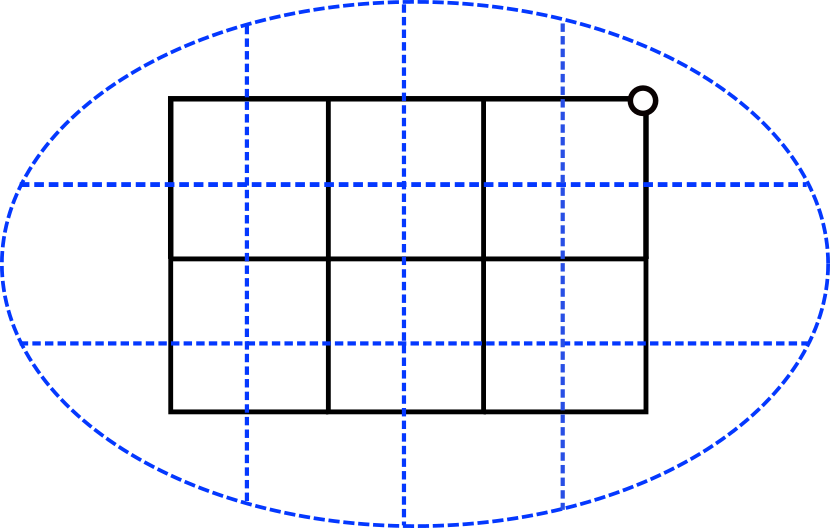
\includegraphics[width=7cm]{figures/grid_dual.png}
  	\caption{Grid Graph and its Dual}
	\label{fig:grid}
 	 \end{center}
\end{figure}

Consider a planar, bipartite graph $G = (V,E)$ and its dual $G^* = (V^*, E^*)$. Distinguish a vertex $v_0 \in V$ and let $v_\infty \in E^*$ represent the ``outside'' vertex from $G$. Considering $G$ as a compact subspace of $\mathbb{R}^2$, we can consider $v_\infty$ to be the point $\infty$ in the one point compactification $\mathbb{R}^2 \cup \{\infty\}$. 

The case that $G$ is a $2 \times 3$ grid is shown in the Figure \ref{fig:grid}. There, $G$ is drawn with solid lines and $G^*$ is drawn with dotted lines. The distinguished vertex $v_0$ is shown with an open circle. The vertex $v_\infty$ is represented by the outermost oval. 



Pick a spanning tree $T$ for $G$ and let $T^*$ be the dual spanning tree for $G^*$. That $T^*$ is dual to $T$ means that the edges of $T$ and $T^*$ do not intersect. It is straightforward to check that $T^*$ always exists. Figure \ref{fig:dualspan} shows $T$ in yellow and $T^*$ in green. 
\begin{figure}[htb!]
	\begin{center}
 	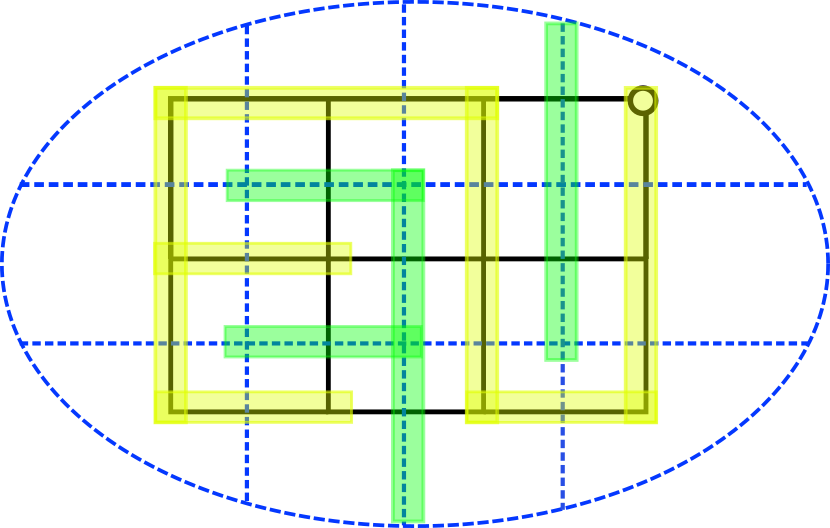
\includegraphics[width=6cm]{figures/grid_dual_trees.png}
  	\caption{Dual Spanning Trees}
	 \label{fig:dualspan}
 	 \end{center}
\end{figure}


\newpage
We now define the \textbf{double graph of $G$} to be the graph $G_d = (V_d, E_d)$ with 
$$
V_d =\left( V \amalg V^* \amalg \{\text{all intersections of an edge $e$ with its dual $e^*$}\} \right) \smallsetminus \{v_0 , v_\infty\}.
$$
The edge set $E_d$ is obtained as a subdivision of $E \amalg E^*$ according to the intersections of each edge with its dual. This process is shown in Figure \ref{fig:dblgraph}, so that each pair $(e,e^*)$ contributes four edges to $E_d$. 
\begin{figure}[htb!]
	\begin{center}
 	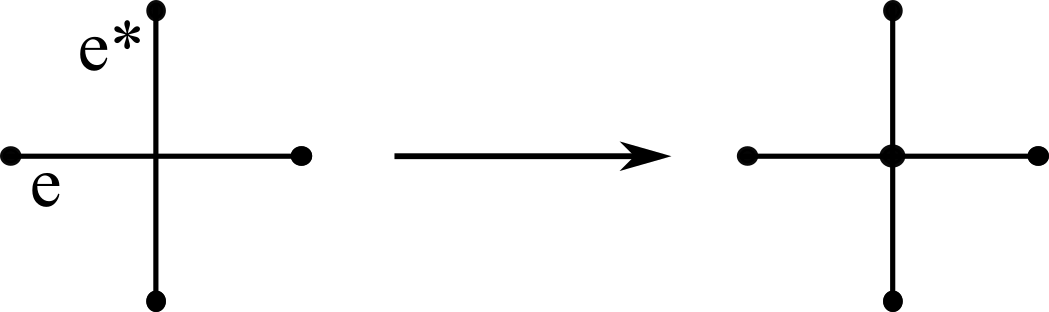
\includegraphics[width=5cm]{figures/grid_subdivid.png}
  	\caption{Subdivision Process for Double Graph}
	\label{fig:dblgraph}
 	 \end{center}
\end{figure}
Note that the definition of $G_d$ depends upon the vertex $v_0$. 

We can now define the correspondence between the spanning trees on $G$ and the perfect matchings on $G_d$. Let $T$ and $T^*$ be as before and identify them with their images in $G_d$. Starting at the leaves of $T$ and $T^*$, match pairs of vertices in $G_d$ along each tree until all vertices are matched. The result will be a perfect matching on $G_d$. 


\begin{figure}[htb!]
	\begin{center}
 	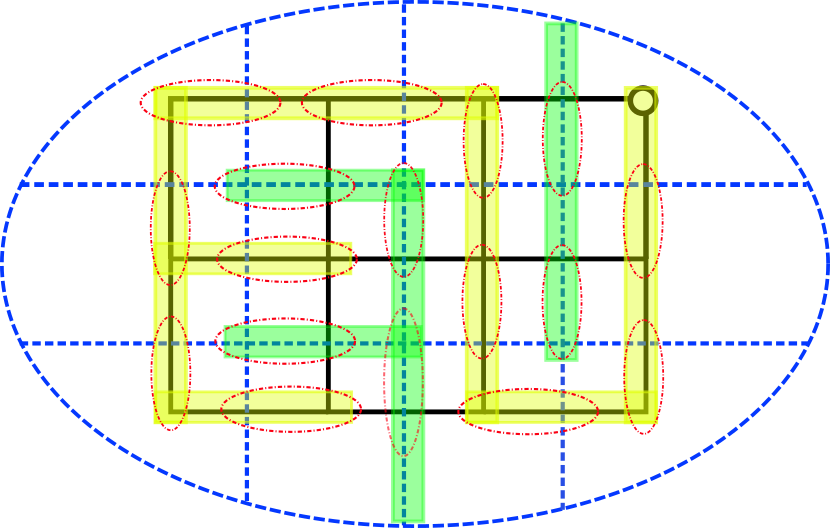
\includegraphics[width=7cm]{figures/grid_double_trees.png}
  	\caption{Subdivision Process for Double Graph}
	 \label{fig:dbltree}
 	 \end{center}
\end{figure}

This process defines a bijection between the spanning trees of $G$ and the perfect matchings of $G_d$. This bijection is due to Temperley. Figure \ref{fig:dbltree} shows the perfect matching on $G_d$ from our example.
	
	
	
	
	
	
\end{document}	
